\documentclass{article}
\usepackage{style}

\begin{document}

% University Logo, Course Name, Professor's Name, Date, Homework Title,
% Homework Number, Student Name, Student Identifier, Source Code
\cover{./UTFPR.png}{Engenharia de Software}{Leonardo Medeiros}{17/02/2025}
{Lista de Exercícios}{3}{Gabriel dos Santos Schmitz}{2487438}
{https://github.com/gabrielzschmitz/uni/tree/main/eng-soft/lista3}

\question{Qual a provável arquitetura dos seguintes sistemas? Justifique
	brevemente sua resposta.}
\subquestion{Microsoft Excel (versão para desktop)}
\answer{
	A arquitetura do Microsoft Excel para desktop é monolítica, com a maior parte
	da lógica e funcionalidade centralizada em um único executável. Isso é comum
	em programas de desktop que não dependem de servidores, exceto para
	sincronização na nuvem ou atualizações.
}
\subquestion{Nubank App (mobile)}
\answer{
	A arquitetura do Nubank App é baseada no modelo cliente-servidor, com o
	aplicativo interagindo com servidores para processar transações e fornecer
	serviços personalizados. Aplicativos financeiros geralmente utilizam
	servidores para garantir segurança e escalabilidade, com comunicação via APIs
	RESTful ou GraphQL.\
}
\subquestion{Twitter Web (front-end)}
\answer{
	A arquitetura do front-end do Twitter Web segue um modelo cliente-servidor,
	onde o navegador interage com APIs para acessar dados e interações. A
	comunicação com os servidores é feita via APIs para garantir uma interface
	rápida e dinâmica.
}
\subquestion{Google Slides (front-end)}
\answer{
	A arquitetura do Google Slides no front-end segue o modelo cliente-servidor,
	com o navegador se comunicando com servidores para salvar e recuperar
	documentos. A aplicação utiliza JavaScript com frameworks modernos e
	armazenamento centralizado no servidor, com suporte limitado a funcionalidades
	offline.
}
\subquestion{Twitter (backend)}
\answer{
	A arquitetura do backend do Twitter é orientada a microsserviços, com
	diferentes componentes para gerenciar feeds, usuários e notificações. Isso
	permite alta disponibilidade e escalabilidade, com uso de filas de mensagens e
	bancos de dados NoSQL para lidar com dados em tempo real.
}
\subquestion{Moodle}
\answer{
	A arquitetura do Moodle segue o modelo cliente-servidor tradicional, com uma
	interface web interagindo com um servidor que gerencia dados de cursos e
	usuários. O Moodle utiliza PHP e bancos de dados relacionais como MySQL ou
	PostgreSQL para persistência de dados.
}

\newpage
\question{Responda sobre microsserviços:}
\subquestion{Por que uma arquitetura baseada em microsserviços oferece
	flexibilidade para os times colocarem seu código em produção de forma
	independente?}
\answer{
	Porque cada microsserviço é independente, permitindo que equipes trabalhem e
	deployem suas mudanças sem afetar outros serviços. Isso facilita atualizações
	contínuas e escalabilidade.
}
\subquestion{Por que isso é menos viável em uma arquitetura monolítica? Ou seja,
	por que não é recomendável que um time, ao fazer uma modificação em um
	monolito, coloque-a em produção imediatamente?}
\answer{
	Em uma arquitetura monolítica, todas as partes do sistema estão fortemente
	interligadas, tornando o deploy de uma modificação arriscado, pois pode afetar
	outras funcionalidades do sistema.
}
\subquestion{Por que microsserviços não devem compartilhar o mesmo BD?}
\answer{
	Porque compartilhar o banco de dados pode criar dependências indesejadas entre
	os microsserviços, dificultando a escalabilidade e a independência de cada
	serviço.
}

\question{Suponha uma empresa de streaming que deseja implementar um
	sistema detector de problemas de qualidade em seus vídeos (por
	exemplo, problemas nas legendas, no áudio, congelamento de imagens,
	etc). Os vídeos estão todos armazenados em um sistema de storage, isto
	é, em memória secundária. A empresa está avaliando duas arquiteturas:
	\begin{itemize}
		\item Arquitetura #1: cada detector é um microsserviço, que recebe o nome do
		      vídeo como parâmetro, carrega o mesmo do storage e executa um
		      algoritmo de detecção de problemas de qualidade nesse vídeo.
		\item Arquitetura #2: os detectores são módulos de um monolito. Então, o
		      vídeo é carregado uma única vez do storage para a memória principal e
		      compartilhado por todos os detectores de qualidade.
	\end{itemize}
	Supondo que a empresa de streaming tem milhões de clientes (ou seja, é
	uma empresa do porte da Amazon Prime Video) qual arquitetura você
	considera mais escalável? Justifique.}
\answer{
	A Arquitetura #1 é mais escalável, pois microsserviços independentes podem ser
	distribuídos e escalados de forma independente, permitindo que a carga de
	trabalho seja balanceada entre vários servidores. Isso facilita o
	gerenciamento de milhões de vídeos simultaneamente, sem sobrecarregar um único
	sistema.
}

\newpage
\question{Em junho de 2021, o seguinte e-mail foi enviado por engano para
	milhares de assinantes da HBO.\ O que deve ter acontecido para que este mail
	chegasse aos usuários finais da HBO?\
	\begin{center}
		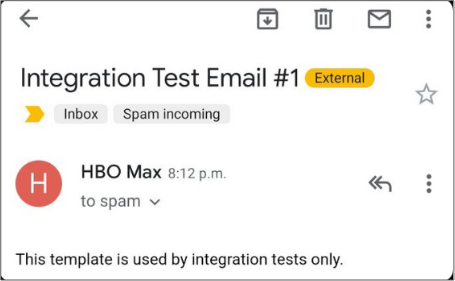
\includegraphics[width=0.5\textwidth]{./fig/hbo-email.png}
	\end{center}
}
\answer{
	O e-mail provavelmente foi enviado por engano devido a uma falha na automação
	dos testes de integração, onde um modelo de e-mail destinado apenas para
	testes foi erroneamente incluído na lista de envio para os assinantes. Isso
	pode ocorrer se os ambientes de produção e testes não forem devidamente
	isolados.
}

\newpage
\question{Suponha a seguinte função: Suponha que você está trabalhando em seu
	repositório local em um código que chama \texttt{`destaca\_texto`}. Descreva
	uma mudança (push) feita nessa função, por outro dev, que:}
\begin{listing}[H]
	\begin{minted}[frame=none, framesep=2mm, baselinestretch=1.2,
    bgcolor=whitesmoke, fontsize=\footnotesize, linenos]{Java}
String destaca_texto(String texto, String palavra) {
// `texto` é um texto em markdown
// pesquisa todas as ocorrências de `palavra` em `texto`
// converte palavra para negrito (palavra, em markdown)
}
  \end{minted}
\end{listing}

\subquestion{causa um erro de compilação no seu código (após um pull)?}
\answer{
	Uma mudança que causa um erro de compilação poderia ser a modificação do
	método \texttt{destaca\_texto} para incluir um tipo de retorno diferente, por
	exemplo, alterando o tipo de \texttt{String} para \texttt{void}, o que
	causaria um erro de compilação ao tentar compilar seu código, pois o seu
	código esperaria um valor de retorno, mas a função não retornaria mais nada.
}
\begin{minted}[frame=none, framesep=2mm, baselinestretch=1.2,
  bgcolor=whitesmoke, fontsize=\footnotesize, linenos]{Java}
void destaca_texto(String texto, String palavra) {
    // código alterado que não retorna mais nada
}
\end{minted}

\subquestion{causa um erro de lógica no seu código (após um pull)?}
\answer{
	Uma mudança que causa um erro de lógica poderia ser a alteração do código da
	função de forma que, ao invés de aplicar o negrito corretamente, ela
	substituísse as ocorrências da palavra por uma string incorreta ou deixasse de
	aplicar o negrito. Isso faria com que o comportamento da função fosse
	inesperado, mas o código compilasse corretamente.

	Neste caso, o erro de lógica pode ser uma falha na formatação do markdown, que
	não resultaria no negrito esperado.
}
\begin{minted}[frame=none, framesep=2mm, baselinestretch=1.2,
  bgcolor=whitesmoke, fontsize=\footnotesize, linenos]{Java}
String destaca_texto(String texto, String palavra) {
    // código alterado com erro de lógica
    texto = texto.replace(palavra, "**" + palavra + "**"); // erro de formatação
    return texto;
}
\end{minted}

\newpage
\question{Defina (e diferencie) os seguintes termos:}
\subquestion{Integração contínua (continuous integration)}
\answer{
	Integração contínua (CI) é o processo de integrar e testar código de forma
	frequente em um repositório compartilhado, para detectar erros mais
	rapidamente.
}
\subquestion{Entrega contínua (continuous delivery)}
\answer{
	Entrega contínua (CD) é o processo de garantir que o código esteja sempre em
	um estado pronto para produção, permitindo a entrega automatizada, mas com uma
	aprovação manual antes do deployment.
}
\subquestion{Deployment contínuo (continuous deployment)}
\answer{
	Deployment contínuo (CD) é a prática de automatizar a entrega do código
	diretamente para produção após passar nos testes, sem intervenção manual.
}

\question{Suponha que você foi contratado por uma empresa que fabrica
	impressoras. E que ficou responsável por definir as práticas de DevOps
	adotadas no desenvolvimento dos drivers dessas impressoras. Qual das seguintes
	práticas você adotaria nesse desenvolvimento: deployment contínuo ou delivery
	contínuo? Justifique.}
\answer{
	Eu adotaria entrega contínua (continuous delivery), pois permite que os
	drivers estejam sempre prontos para produção, garantindo maior controle e
	segurança antes do deployment, o que é importante para hardware como
	impressoras.
}

\question{Linguagens como C possuem suporte a diretivas de compilação
	condicional do tipo #ifdef e #endif. Qual a diferença entre elas e feature
	flags?}
\answer{
	A diferença é que as diretivas de compilação condicional (\#ifdef, \#endif)
	controlam a inclusão de partes do código na compilação, enquanto as feature
	flags são usadas em tempo de execução para ativar ou desativar funcionalidades
	específicas.
}

\question{No contexto de TBD, feature flags são usadas para desabilitar
	implementações que ainda não estão prontas. Porém, fora do contexto de TBD,
	feature flags podem ser usadas para habilitar ou desabilitar features
	“prontas” de um sistema. Dê um exemplo de um sistema e de algumas de suas
	features que podem ser ligadas ou desligadas.}
\answer{
	Exemplo: Em um sistema de e-commerce, algumas features como `desconto para
	novos usuários' ou `recomendações personalizadas' podem ser controladas por
	feature flags, permitindo ativá-las ou desativá-las sem alterar o
	código-fonte.
}

\question{Qual a principal diferença entre um teste A/B e um release canário?}
\answer{
	A principal diferença é que o teste A/B testa diferentes versões de uma
	feature com grupos de usuários distintos, enquanto o release canário envolve
	liberar uma nova versão para um pequeno grupo de usuários antes de um
	lançamento completo.
}

\newpage
\question{Complete supondo uma empresa que usa git-flow.}
\answer{
	\begin{tabular}{l l l}
		\toprule
		\textbf{Tipo de Branch} & \textbf{Branch de Origem} & \textbf{Branch(es) de Destino} \\
		\midrule
		Feature                 & develop                   & develop, master                \\
		Release                 & develop                   & master                         \\
		Hotfix                  & master                    & master, develop                \\
		\bottomrule
	\end{tabular}
}

\question{Suponha que você ficou responsável por implementar uma mudança em uma
	função \texttt{f}. E, para isso, você decidiu usar uma estratégia de `branch
	por abstração'. Para isso, você criou uma cópia de \texttt{f}, chamada
	\texttt{f\_novo}. Suponha ainda que \texttt{f} chama uma função \texttt{g}.}
\subquestion{Se um bug for corrigido em \texttt{g}, por um outro desenvolvedor,
	qual comando git você deve usar para obter a versão corrigida de \texttt{g}?}
\answer{
	Você deve usar o comando \texttt{git merge} para incorporar a versão corrigida
	de \texttt{g} da branch onde o bug foi corrigido para a sua branch.
}
\subquestion{Agora suponha que sua mudança em \texttt{f} exija uma mudança
	também em \texttt{g}. O que você deveria fazer nesse caso?}
\answer{
	Você deve atualizar a função \texttt{g} em sua branch, criando uma nova versão
	dela, ou então fazer um \texttt{git merge} para incluir as mudanças de
	\texttt{g} na sua branch, antes de atualizar a função \texttt{f\_novo}.
}

\end{document}
